\section{Dispositif: L'arche cosmique}
\label{sect:Muon_arche}

Cette expérience a pour objectif la mesure de la distribution angulaire des muons atmosphériques.
Au cours de ce laboratoire, vous apprendrez à utiliser et caractériser des scintillateur et photomultiplicateurs dans le cadre de la détections de muons.
Vous calibrerez le dispositif et développerez la logique d'acquisition des données.
Finalement, vous analyserez celles-ci grâce aux outils statiques vus au cours théorique.

\subsection{Agenda du laboratoire}
\begin{tabular}{p{0.2\linewidth} p{0.8\linewidth}}
Lundi & - Familiarisation avec le matériel\newline
		- Vérification des signaux analogiques des PMs à l'oscilloscope\newline
		- Mise en temps des signaux\newline
		- Mesure de l'efficacité des PMs en fonction de la tension et du seuil\\

Mardi & - Mesure de l'efficacité des PMs en fonction de l'angle zénithal\newline
		- Introduction au TDC et \textit{dual-timer}\newline
		- Éventuellement, première calibration de la position en fonction de la différence de temps d'arrivée des signaux\\

Mercredi & - Calibration de la position en fonction de la différence de temps d'arrivée des signaux\newline
		- Mesure de la vitesse de la lumière dans les guides de lumières\newline
		- Début de l'acquisition de données\\

Jeudi et Vendredi & - Mise en forme, préparation des données\newline
		- Développement d'une simulation Monte-Carlo\newline
		- Développement du programme d'analyse\newline
		- Préparation de la présentation\\
\end{tabular} 

\subsection{Dispositif expérimental}

\begin{figure}
\begin{center}
    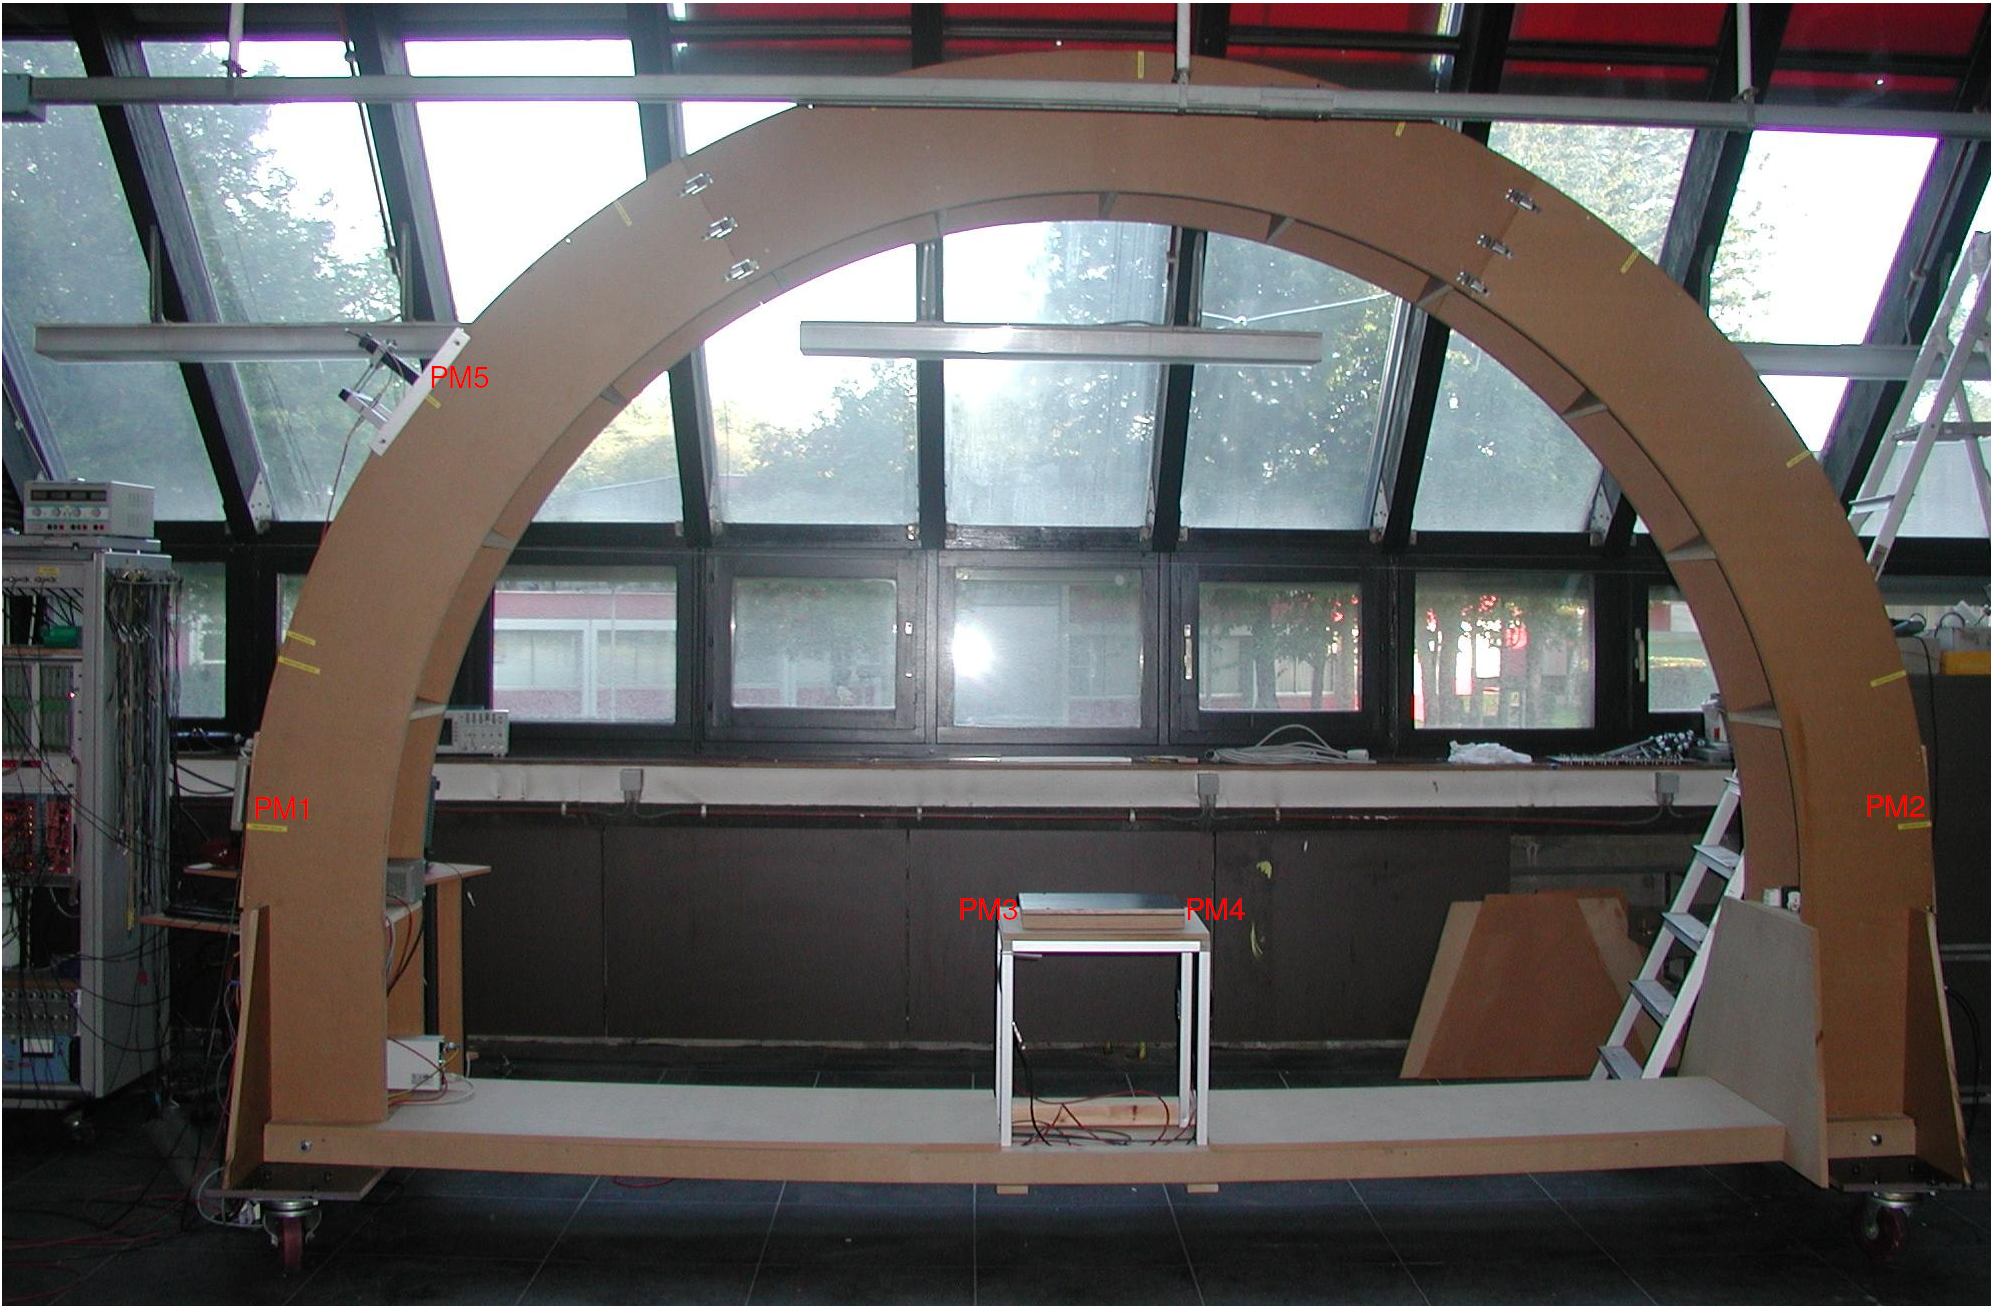
\includegraphics[width=0.75\textwidth]{figures/dispositif_arche.png}
\end{center}
\caption{Photo du dispositif de l'arche précisant la localisation des photomultiplicateurs}
\label{fig:dispositif_arche}
\end{figure}

L'arche, dont la photo est visible sur la figure~\ref{fig:dispositif_arche}, est constituée d'un demi cercle recouvert de blocs scintillants.
Plusieurs guides de lumière (ou \textit{wavelength shifter}) transmettent la lumière produites par scintillation jusqu'aux photomultiplicateurs situés aux pieds de l'arche (PM1\&PM2).
Au centre de celle-ci est installé un autre scintillateur lu par deux photomultiplicateurs (PM3\&PM4).
Ces quatre photomultiplicateurs permettent de sélectionner des muons passant à la fois par le plan et le centre de l'arche.
En mesurant la différence de temps entre l'arrivée des signaux sur les PM1\&PM2, il est possible d'extraire l'angle d'incidence du muon détecté.
Un cinquième scintillateur accompagné de son photomultiplicateur (PM5) ainsi que des LEDs installées le long de l'arche complètent le dispositif à des fins de calibration.

Les dimensions, qui vous aideront lors de l'analyse des données, sont les suivantes:
\begin{itemize}
    \item Dimension des scintillateurs PM3, PM4 \& PM5: \(\SI{21}{\cm}\textrm{ x }\SI{21}{\cm}\)
    \item Largeur des blocs scintillants sur l'arche: \(\SI{21}{\cm}\)
    \item Longueur des blocs scintillants sur l'arche: \(\SI{517}{\cm}\)
    \item Diamètre de l'arche: \(\SI{398.3}{\cm}\)
\end{itemize}

\subsection{Prise de mesures}
L'expérience aura été préalablement préparée de sorte à ce que le matériel soit fonctionnel à proximité immédiate.
Afin de vous familiarisez avec le dispositif et de lancer l'acquisition des données, il vous est demandé de suivre les étapes suivantes:

\begin{center}
\fbox{
\begin{minipage}{0.75\textwidth}
    \textbf{Se familiariser avec le dispositif :} 
    \begin{itemize}
        \item Vérifier le signal des différents PMs
        \item Étudier l'efficacité d'un PM
        \item Mesurer l'efficacité angulaire de l'arche
        \item Mesurer la relation entre la position et la différence de temps
        \item Préparer la prise de données
    \end{itemize}
\end{minipage}
}
\end{center}

\subsubsection{Mise en route du dispositif}

Après avoir mis sous tension les PMs, essayez d'observer des signaux sur chacun d'entre eux à l'aide de l'oscilloscope.
Correspondent-il à ce à quoi vous vous attendez ?
Essayez d'observer des coincidences.
Une fois le fonctionnement des PMs établi, utilisez les discriminateurs pour convertir les signaux analogiques en signaux numériques.

\textit{Pour gagner du temps, vous pouvez régler immédiatement la tension du PM5 sur \(\SI{1100}{V}\) et le seuil de son discriminateur sur \(\SI{-80}{\mV}\).}

\paragraph{Attention} Veillez à ne pas dépasser la tension de \(\SI{900}{V}\) sur les PM3\&PM4 pour de pas les endommager.

\subsubsection{Mesure d'efficacité}
Afin de mieux comprendre le comportement des PMs et de les régler au mieux, vous devez mesurer leur efficacité en fonction de la tension d'alimentation et du seuil du discriminateur.
Cette opération se déroule en deux étapes.
Dans un premier temps, faites varier le seuil du discriminateur jusqu'à atteindre le plateau d'efficacité.
Une fois le seuil idéal sélectionné, répétez l'opération, mais en faisant varier la tension cette fois.
Si vous avez suffisamment de temps, il vous est possible de répéter la première mesure pour la nouvelle tension d'alimentation.

De quels PMs allez-vous mesurer l'efficacité ?
Comment allez-vous utiliser la logique NIM ?
N'oubliez pas de mesurer le taux d'événements détectés par le PM en cours de test.

\ifthenelse{\boolean{showAdditional}}{
\begin{additional}
    La mesure de l'efficacité du PM5 est rendue délicate par la présence de fausses coincidences entre les PM3\&PM4.
    Dans le cadre de se laboratoire, il est préférable de mesurer les efficacités des PM3\&PM4 (simultanément si besoin pour gagner du temps).

    \bigskip

    Les opérations logiques à implémenter sont les suivantes:
    \begin{itemize}
        \item Output 1: PM3\&PM5
        \item Output 2: PM4\&PM5
        \item Output 3: PM3\&PM4\&PM5 (attention, cette condition implique les deux conditions précédentes)
    \end{itemize}

    \bigskip

    Ces signaux, ainsi que les signaux en sortie des discriminateurs, doivent être comptés grâce au \textit{scaler}.

    % \begin{figure}
    % \begin{center}
    %     \includegraphics{figures/arche_pm3_pm4.png}
    % \end{center}
    % \caption{Caractérisation de PM3\&PM4 de l'arche}
    % \label{fig:arche_pm3_pm4}
    % \end{figure}
\end{additional}
}

\subsubsection{Mesure de l'efficacité angulaire}

Cette expérience est basée sur le comptage d'événements fonction de l'angle d'incidence des muons atmosphériques.
En conséquence, toute différence d'efficacité dépendante de l'angle doit être corrigée.

Maintenant que les seuils de fonctionnement pour les PM3, PM4 \& PM5 sont établis, vous allez devoir:
\begin{enumerate}
    \item Trouver les seuils optimaux pour les PM1\&PM2 en suivant la procédure utilisée précédemment. \textit{Les tensions d'alimentation ne sont pas réglables.}
    \item Mesurer l'efficacité des PM1\&PM2 pour différents angles d'incidence. Calculer l'efficacité angulaire totale.
\end{enumerate}

Mesurez-vous l'efficacité angulaire de manière optimale ?
Comment utilisez-vous cette information dans votre analyse ?

\ifthenelse{\boolean{showAdditional}}{
\begin{additional}
    La mesure d'efficacité angulaire n'est pas optimale dans notre cas.
    Par manque de temps, la mesure d'efficacité est effectuée en utilisant tous les angles d'incidence alors que la mesure finale n'utilise que les muons normaux à l'arche. 

    En fonction de la manière d'analyser les données, la correction est plus ou moins facile à appliquer.
    Si les données sont mises en boite, il suffit de donner un poids égal à l'inverse de l'efficacité pour chaque événement.
    Si les données ne sont pas mises en boîte, la fonction à ajuster doit être multipliée par l'efficacité point par point.

    D'habitude les résultats ne sont pas nettement améliorés lorsque la correction est appliquée.
    Implémenter cette correction ne devrait se faire que si le temps le permet.

    \begin{center}
        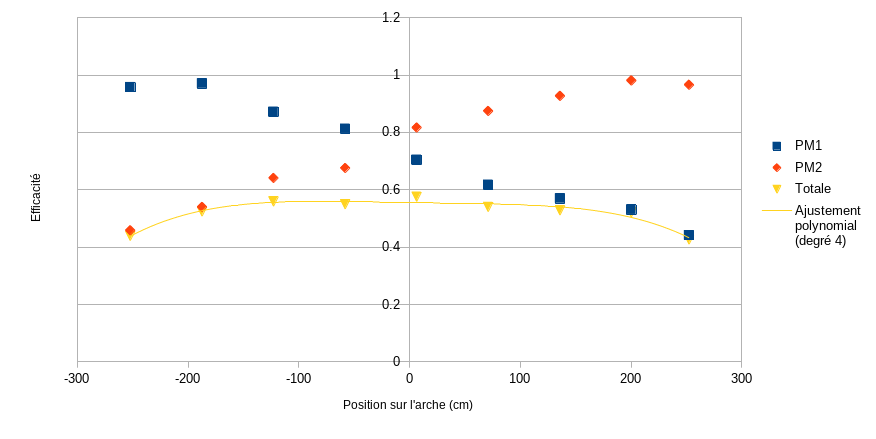
\includegraphics[width=0.7\textwidth]{figures/arche_eff_angulaire.png}
        \\ Efficacité en fonction de l'angle zénithal
    \end{center}
\end{additional}
}

\subsubsection{Calibration de la position en fonction de la différence de temps}

La dernière étape avant la prise de donnée consiste en la mesure de la relation entre la différence de temps d'arrivée des signaux des PM1\&PM2 et la position le long de l'arche.
À cette fin, 15 LEDs ont été insérées dans les blocs scintillants placés le long de l'arche.
Les modules NIM présents vous permettent de pulser individuellement chacune des LEDs.
Le module TDC VME permet de mesurer des temps avec une résolution de \(\SI{25}{\ps}\) dans une fenêtre réglable autour d'un signal de déclenchement (\textit{trigger})\footnote{Plus de documentation sur les réglages de ce modèle de TDC vous est fournie durant le laboratoire.}.

Comment allez-vous faire pulser les LEDs?
Comment réglez-vous la fenêtre d'acquisition du TDC?
Quel \textit{trigger} utilisez-vous?

\ifthenelse{\boolean{showAdditional}}{
\begin{additional}
    En utilisant les deux unités du module \textit{dual-timer}, il est possible de générer un signal de période et de rapport cyclique voulus.
    Pour se faire, il faut connecter la sortie \textit{end-marker} à l'entrée \textit{start} pour chacune des deux unités.
    Les caractéristiques du signal se vérifient facilement à l'oscilloscope.
    Attention à utiliser une fréquence de pulsation suffisamment basse afin de ne pas saturer la lecture du TDC !

    Le \textit{trigger} idéal est dans ce cas ci le signal de commande des LEDs.
    La fenêtre est établie en visualisant les signaux à l'oscilloscope.

    % \begin{figure}
    % \begin{center}
    %     \includegraphics{figures/arche_tdc_led4.png}
    % \end{center}
    % \caption{Exemple de distribution temporelle pour la LED4}
    % \label{fig:arche_tdc_led4}
    % \end{figure}

    % \begin{figure}
    % \begin{center}
    %     \includegraphics{figures/arche_vitesse_lumiere.png}
    % \end{center}
    % \caption{Position sur l'arche en fonction de la différence de temps mesurée}
    % \label{fig:arche_vitesse_lumière}
    % \end{figure}
\end{additional}
}

\subsubsection{Prise de données}

La prise de données constitue la dernière étape de la manipulation.
Pour cela vous devrez définir la logique d'acquisition et l'implémenter les modules NIM et VME.
Celle-ci est similaire à la logique que vous avez développée au point précédent: il vous faut mesurer la différence de temps d'arrivée des signaux des PM1\&PM2.
Dans ce cas ci, nous nous intéressons à des muons atmosphériques qui passent simultanément par le plan et le centre de l'arche. Pourquoi ?

Quelle logique allez-vous implémenter ?
Quels réglages utilisez-vous pour le TDC ?

\ifthenelse{\boolean{showAdditional}}{
\begin{additional}
    La logique fournissant le \textit{trigger} est une coincidence entre les PM1\&PM2\&PM3(4)\&PM5.
    Ainsi, on est assuré de sélectionner des muons étant passés, et ayant été mesurés, à la fois par le plan et le centre de l'arche.
    Cette configuration est évidente pour mesurer un angle zénithal, on peut voir l'arche comme un rapporteur géant.

    Pour ne pas perdre d'événements, il faut faire particulièrement attention à deux points:
    \begin{enumerate}
        \item Les signaux doivent être correctement mis en temps.
              Ceci est complexifié par le fait que les temps d'arrivée des PM1\&PM2 varient événement par événement.
              Les largeurs des fenêtres en sortie des discriminateurs doivent donc être suffisamment grandes.
        \item La fenêtre d'acquisition du TDC doit être correctement configurée.
              Observer les signaux de tous les PMs se révèle être une aide précieuse dans cet objectif.
    \end{enumerate}

    % \begin{figure}
    % \begin{center}
    %     \includegraphics{figures/arche_distribution.png}
    % \end{center}
    % \caption{Distribution des différences de temps mesurées (aucune correction appliquée)}
    % \label{fig:arche_distribution.png}
    % \end{figure}
\end{additional}
}

\subsection{Analyse des données}

A présent, nous pouvons nous concentrer sur l'analyse des données afin de vérifier la loi en \(\cos^2(\theta)\).
En vous basant sur l'ensemble de vos données, il vous est demandé de calculer:

\begin{center}
\fbox{
\begin{minipage}{0.75\textwidth}
    \textbf{Arche cosmique :}
    \begin{itemize}
        \item La vitesse de la lumière dans le guide de lumière
        \item La puissance \(\alpha\) et l'alignement \(\theta_0\) dans la loi \(\cos^{\alpha}(\theta-\theta_0)\)
    \end{itemize}
\end{minipage}
}
\end{center}
